%------------------------------------------------------------------------------
% Template file for the submission of papers to IUCr journals in LaTeX2e
% using the iucr document class
% Copyright 1999-2013 International Union of Crystallography
% Version 1.6 (28 March 2013)
%------------------------------------------------------------------------------

\documentclass[preprint]{iucr}              % DO NOT DELETE THIS LINE
%%\documentclass{iucr}              % DO NOT DELETE THIS LINE
\usepackage{graphicx}
\usepackage{url}

     %-------------------------------------------------------------------------
     % Information about journal to which submitted
     %-------------------------------------------------------------------------
     \journalcode{J}              % Indicate the journal to which submitted
                                  %   A - Acta Crystallographica Section A
                                  %   B - Acta Crystallographica Section B
                                  %   C - Acta Crystallographica Section C
                                  %   D - Acta Crystallographica Section D
                                  %   E - Acta Crystallographica Section E
                                  %   F - Acta Crystallographica Section F
                                  %   J - Journal of Applied Crystallography
                                  %   M - IUCrJ
                                  %   S - Journal of Synchrotron Radiation

\begin{document}                  % DO NOT DELETE THIS LINE

     %-------------------------------------------------------------------------
     % The introductory (header) part of the paper
     %-------------------------------------------------------------------------

     % The title of the paper. Use \shorttitle to indicate an abbreviated title
     % for use in running heads (you will need to uncomment it).

\title{The NeXus Data Format}
%\shorttitle{Short Title}

     % Authors' names and addresses. Use \cauthor for the main (contact) author.
     % Use \author for all other authors. Use \aff for authors' affiliations.
     % Use lower-case letters in square brackets to link authors to their
     % affiliations; if there is only one affiliation address, remove the [a].
\cauthor[a]{Mark}{K\"onnecke}{mark.koennecke@psi.ch}

\author[b]{Frederick A.}{Akeroyd}

\author[c]{Herbert J.}{ Bernstein}

\author[d]{Aaron S.}{ Brewster}

\author[e]{Stuart I.}{ Campbell}

\author[f]{Bj{\o}rn}{ Clausen}

\author[b]{Stephen}{ Cottrell}

\author[g]{Jens Uwe}{ Hoffmann}

\author[h]{Pete R.}{ Jemian}

\author[i]{David}{ M\"annicke}

\author[j]{Raymond}{Osborn}

\author[e]{Peter F.}{ Peterson}

\author[k]{Tobias}{Richter}

\author[l]{Jiro}{ Suzuki}

\author[m]{Benjamin}{ Watts}

\author[n]{Eugen}{ Wintersberger}

\author[o]{Joachim}{ Wuttke}

\aff[a]{Laboratory for Development and Methods, Paul Scherrer Institute, 5232 Villigen-PSI, \country{Switzerland}}
\aff[b]{ISIS Facility, STFC, Rutherford Appleton Laboratory, Didcot, OX11 0QX, \country{UK}}
\aff[c]{imgCIF, Dowling College, Shirley, NY 11769, \country{USA}}
\aff[d]{Lawrence Berkeley National Laboratory, Berkeley, CA 94720, \country{USA}}
\aff[e]{Spallation Neutron Source, Oak Ridge National Laboratory, Oak Ridge, TN 37831, \country{USA}}
\aff[f]{Los Alamos National Laboratory, Los Alamos, NM 87545, \country{USA}}
\aff[g]{Helmholtz Zentrum, 14109 Berlin, \country{Germany}}
\aff[h]{Advanced Photon Source, Argonne National Laboratory, Argonne, IL 60439, \country{USA}}
\aff[i]{ANSTO, New South Wales 2234, \country{Australia}}
\aff[j]{Argonne National Laboratory, Argonne, IL, 60439, \country{USA}}
\aff[k]{Diamond Light Source, Oxfordshire OX11 0DE, \country{UK}}
\aff[l]{KEK, Ibaraki 305-0801, \country{Japan}}
\aff[m]{Swiss Light Source, Paul Scherrer Institute, 5232 Villigen-PSI, \country{Switzerland}}
\aff[n]{Deutsches Elektronen-Synchrotron DESY, 22607 Hamburg, \country{Germany}}
\aff[o]{Forschungszentrum J\"ulich, JCNS at MLZ, 85747 Garching, \country{Germany}}


     % Use \shortauthor to indicate an abbreviated author list for use in
     % running heads (you will need to uncomment it).

%\shortauthor{Soape, Author and Doe}

     % Use \vita if required to give biographical details (for authors of
     % invited review papers only). Uncomment it.

%\vita{Author's biography}

     % Keywords (required for Journal of Synchrotron Radiation only)
     % Use the \keyword macro for each word or phrase, e.g. 
     % \keyword{X-ray diffraction}\keyword{muscle}

%\keyword{keyword}

     % PDB and NDB reference codes for structures referenced in the article and
     % deposited with the Protein Data Bank and Nucleic Acids Database (Acta
     % Crystallographica Section D). Repeat for each separate structure e.g
     % \PDBref[dethiobiotin synthetase]{1byi} \NDBref[d(G$_4$CGC$_4$)]{ad0002}

%\PDBref[optional name]{refcode}
%\NDBref[optional name]{refcode}

\maketitle                        % DO NOT DELETE THIS LINE

\begin{synopsis}
Description of the NeXus data format for x-ray and neutron scattering and muSR
\end{synopsis}

\begin{abstract}
NeXus is an effort by an international group of scientists to define 
 a common data exchange and archival format for neutron, X-ray, and muon experiments.   
NeXus is built on top of the scientific data format HDF5 and adds 
domain-specific 
rules for organizing data within HDF5 files in addition to a dictionary of well-defined 
domain-specific field names. The NeXus data format has two purposes.  First, NeXus defines a
format that can serve as a container for all relevant data associated
with a beamline. This is a very important use case.  Second, NeXus
defines standards in the form of \emph{application definitions} for the
exchange of data between applications.  NeXus provides structures for raw experimental data as well as for processed data.  
\end{abstract}


 \section{Introduction}

Increasingly, major neutron and X-ray facilities have chosen to store data using the NeXus data format. 
Since the last publication dating from 2006, NeXus\cite{nxold} has undergone substantial refocusing, 
refinement and enhancement as described in this paper.  

Historically, neutron and X-ray facilities have chosen to store data in a plethora of 
home-grown data formats. This scheme has a number of drawbacks addressed by NeXus: 
\begin{itemize}
\item It makes the life of traveling scientists unnecessarily difficult as they must deal with multiple files 
 in different formats, file converters and such in order to extract scientific information from the data.
 \item An unnecessary burden is imposed on data analysis software producers to accommodate many different formats.  
\item The whole idea of open access to data is sabotaged if the data is in a format which cannot be easily understood.
\item Scientific integrity is jeopardized if the data cannot be understood or important elements are missing.
\item Modern high speed detectors produce data at such a high rate that many older single image storage schemes 
 have become impractical and 
 an efficient container format is mandatory.
\end{itemize}

The primary necessity for a data format is to define a physical file format: how is the data written to disk? Rather than invent
yet another format, NeXus chose HDF5\cite{hdf5} as the physical file format. 
HDF5 is a binary file format in the public domain and is well supported by both commercial and free software tools. It  
is efficient, self-describing, and platform-independent.

NeXus data files are built using basic HDF5 storage elements: 
data groups (like file system folders), 
data fields (such as strings, floats, integers, and arrays), 
attributes (additional descriptors of groups and fields), 
and links (like file system links).  NeXus is implemented in terms 
of these basic storage elements.


NeXus adds to HDF5:
\begin{itemize}
\item Rules for organizing domain-specific data within a HDF5 file. Most notably a data hierarchy for arranging data in the file.
\item A link structure to enable quick default visualization
\item A dictionary of documented domain-specific fields expressed in the form of \emph{base classes}
\item Definitions of standards that can be validated in the form of \emph{application definitions}
\end{itemize}

The development of NeXus is overseen by a committee, the NeXus International Advisory Committee (NIAC)\cite{niac}.

\section{General Principles}

The authors of data-acquisition and instrument-control software are encouraged to generate exactly \emph{one} NeXus container file per measurement
(a measurement is either a data accumulation under fixed conditions
or a scan).
This file includes not only the detector and monitor data,
but also metadata, information on the state of the beamline, parameter logs, and more.
Authors of data-reduction and data-analysis software can use NeXus to
store processed data along with metadata and a processing log.

NeXus can be used for many different experimental techniques, and at different levels of 
data processing. For each of these different applications,
a specific subset of the standardized NeXus entities 
(data groups and fields) is needed. The minimum set of fields for a particular 
use case is standardized in the NeXus application definitions (Sect.~\ref{sect_appdef}). 
The minimum set can always be enhanced by adding additional fields from the NeXus base classes (Sect.~\ref{sect_base}). 

As a container format, NeXus allows files to be extended at any moment by
additional content, including NeXus base classes, HDF5 groups, and HDF5 datasets.
Because HDF5 provides full read-write access to the file, such changes can
be made in an existing NeXus file without the need to write a complete new file.

The combination of a well-defined hierarchy of groups with a comprehensive and well-documented dictionary of data and metadata names ensures
that NeXus files are self-describing. It should be possible for another scientist to understand the contents of a NeXus file without consulting 
documentation specific to any one facility or beamline. By enabling the storage of comprehensive metadata, the NeXus format facilitates the 
sharing of data between collaborators and long-term data curation. 



\section{Data File Hierarchies}

NeXus uses a group hierarchy for arranging data in an HDF5 file.  Data files may contain raw data or processed data or both, each of which has a hierarchy.  

\subsection{Raw Data File Hierarchy}


The major focus of NeXus has been the recording of \emph{raw} experimental data, i.e. information taken directly from the experimental 
equipment or processed only as required to provide physically meaningful values.
The NeXus raw data file hierarchy is the consequence of some practical considerations. 
An overview of the NeXus data file structure for raw experimental data is shown in FIG.~\ref{rawfile}.


When looking at a beamline it is easy to 
discern different components: beam optic components, sample position, detectors and such. It is quite natural to replicate this physical 
separation with a logical arrangement of storing the data from each component into a separate group. This approach explains the 
list of beamline components in the \textit{NXinstrument} group presented in FIG.~\ref{rawfile}. 
As there can be multiple instances of the same kind of equipment, such as slits or detectors, in a given beamline it becomes necessary
to add type information to the group name. This type information, the NeXus class name, is provided by a HDF5 attribute.
By convention NeXus class names start 
with the prefix \textit{NX}. Each NeXus group describing a beamline component contains further groups and fields describing the component. 
A field can contain a single number, a text string or an array, as appropriate to the data to be described.  

The need to be able to store multiple related scans or runs in the same file, or to capture 
a complete workflow in a file, causes the beamline component hierarchy to be pushed one level deeper into an \textit{NXentry} 
group in the hierarchy. The \textit{NXentry}  group thus represents one scan or run (or a processed data entry, as will be discussed later). 
The \textit{NXentry} group also holds the experiment metadata, such as the date and time at which it was performed. 

In the course of the evolution of NeXus,
the decision was taken to move \textit{NXmonitor}
out of \textit{NXinstrument} to the higher hierarchy level of \textit{NXentry},
in order to facilitate quick inspection by humans.

To enable a simple default visualization,
an \textit{NXdata} group must be provided at \textit{NXentry} level.
It contains information about plot axes and links to the data
(which typically reside in the \textit{NXdetector} group).
Links are supported by HDF5 and work like hard links in the Unix file system.

A special base class, \textit{NXcollection}, exempts its contents from validation
and thereby allows inclusion of any data in arbitrary non-NeXus formats.

\subsubsection{Multiple Method Instruments}

Particularly at X-ray sources,
some instruments offer multiple techniques that can be used in parallel.
For example, small-angle scattering and powder diffraction 
can be measured simultaneously at a SAXS/WAXS beamline.
We recommend storing the data from all methods in \emph{one} file,
in a \emph{single} \textit{NXentry} hierarchy
(FIG.~\ref{multimethod}). All information from all detectors, logs and 
such are collected in this one \textit{NXentry} group to keep the data together.
Information that is particular for one experimental technique
is linked  into a \textit{NXsubentry}. The \textit{NXsubentry} follows the hierarchy of 
\textit{NXentry}, but it will typically only link to the data required by the 
application definition for the specific experimental technique. The point of this scheme 
is that both humans and computerized users can easily locate method-specific data while 
maintaining the full view of the experiment.   


\subsubsection{Scans}

Scans come in all shapes and sizes. Almost anything can be scanned against anything. 
An additional consideration is that, in practice, the final number of scan points in the scan 
cannot be known in advance since it is possible that a scan may be interrupted or terminated
before its planned number of observations. 
Thus, it is a challenge to standardize a scan.
NeXus addresses this challenge through use of HDF5 \emph{unlimited dimensions} and
additional conventions as described below.
With the HDF5 
unlimited dimensions feature, one axis of the data is allowed to expand without limit.  
Thus, the size of a data array does not need to be declared in advance. 
Data can be appended to an array along the unlimited dimension as required. 

Scans are stored in NeXus following these conventions: 
\begin{itemize}
\item Each variable varied or collected in the scan is stored at its appropriate place in the NeXus beamline 
 hierarchy as an array. The arrays first dimension is the scan axis. This is the unlimited dimension in 
 the implementation and data at each scan point is appended to the array. 
\item The \textit{NXdata} group holds links to all the variables varied or collected during the scan. 
 This creates something equivalent to, or better than, the tabular representation people are accustomed to for scans. 
 The detector data can be plotted against any scanned parameter as well as against everything that was 
 deemed worth recording in addition to that.  The necessary data is all gathered together in the \textit{NXdata}
 group either directly or via links, so that other groups do not
 normally have to be searched to do this plotting.
 
\end{itemize}

NeXus also allows multi-dimensional scans. This makes it very simple to produce meaningful slices through data 
volumes even with NeXus-agnostic software ({\it e.g.} HDFView\cite{hdfview}). 

\subsection{Processed Data File Hierarchy}

At the request of the user community, NeXus created a simplified structure for storing the results of data 
processing: be it reduction or analysis. 
An overview of the NeXus structure for processed data is given in FIG.~\ref{procfile}. 


The hierarchy is much reduced as it is not important to carry all experimental information in the data 
reduction. In contrast to the raw data file structure, \textit{NXdata} in the processed file structure is the place 
to store the results of the processing, together with its associated axes if the result is a multi-dimensional array.  

In addition to the \textit{NXdata} and \textit{NXsample} groups, 
the \textit{NXprocess} group provides structure to store details 
about the processing, such as the program (or programs) used, its version, 
the date of processing, and other metadata. 
The \textit{NXprocess} group can hold additional \textit{NXparameter} groups which are containers 
for storing the input and output parameters of the program used to perform the processing. 

\section{Coordinate Systems, Positioning of Components and Further Rules}

For data reduction, it is often necessary to know the exact position and orientation of beamline components. 
The first thing needed is a reference coordinate system. NeXus chose to use the same coordinate system as the 
neutron beamline simulation software McStas\cite{mcstas}. 

For describing the placement and orientation of components, NeXus stores the same information as is used for the 
same purpose in the Crystallographic Interchange Format (CIF)\cite{ITCVG}. CIF (and NeXus) stores the details 
of the translations and rotations necessary to move a given component from the zero point of the coordinate 
system to its actual position. As coordinate transformations are not commutative, the order of transformations 
must also be stored.

Consult the NeXus manual for further rules on the handling of axes, units and special cases of data storage.

\section{Base Classes}
\label{sect_base}

As can be seen from the discussion of the NeXus file hierarchy, 
NeXus arranges data in groups which have a 
type descriptor and a NeXus base class name associated with them.
Technically, the class name is the value of the HDF5 attribute \textit{NX\_class}.
The term \emph{base class} is not used in the same sense as in  
object-oriented programming languages; in particular, there is no inheritance.
The NeXus base classes provide a comprehensive dictionary of terms 
that can be used for each class. 
The terms in the dictionary comprise concepts and names common to the topic of the base class.
The expected spelling and definition of each term is specified in the base classes. 
It is neither expected nor required to provide all the terms specified in a base class. 
These terms designate data fields that can be stored within a group.
A data field can have a simple type (like integer, float, date/time, binary),
or it can be a NeXus subgroup.
The base class definition also contains informal annotations
about the semantics of each field. Terms with other names are permitted but might
not be recognized by standard software.

At base class level, NeXus has no mechanism to mark some fields as obligatory.
\emph{All allowed fields are optional.}
Which of them are written into data files must be decided
according to application needs.
These decisions can be standardized in the form of
application definitions (see below, Sect.~\ref{sect_appdef}).

The NeXus base classes are encoded in NeXus Description Language (NXDL)\cite{nxman}. NXDL is 
just another form of an XML file that specifies the content of a NeXus base class. 
NXDL files may be parsed either by humans or by software and 
may be validated for syntax and content.  The NXDL files are used to validate the structure of
NeXus data files. Java source code of a GUI tool has been prepared\cite{nxvalidate} to perform such validation.


\section{Application Definitions}
  \label{sect_appdef}

An application definition, expressed in NXDL, specifies a data structure
for a given application domain such as a scientific technique or a specific type of instrument.
The data structure consists of a hierarchy of NeXus groups.
For each group, a \emph{minimum} content is specified.
Application definitions are therefore different than
base class definitions, which specify a comprehensive 
dictionary of terms that can be used.

Historically, an application definition addressed one type of instrument,
like X-ray reflectometer, or direct-geometry neutron time-of-flight spectrometer.
Thus, application definitions were originally named \emph{instrument definitions}.
However, as NeXus can also be used for processed data
like a tomographic reconstruction or a dynamic scattering law $S(Q,\omega)$, 
the more generic term \emph{application definition} has been adopted.


\section{Contributed Definitions}
  \label{sect_contribdef}

The process of drafting and ratifying application definitions
is ongoing (see also below, Sect.~\ref{sect_gov}).
Currently, scientists representing both
the NeXus International Advisory Committee and the IUCr Committee on the Maintenance
of the CIF standard 
are nearly finished with a NeXus application definition for macromolecular crystallography.
CBFlib\cite{cbflib} is being extended to work with NeXus-MX format. This work will be published in another paper. 
Work on another NeXus application definition for reduced small-angle scattering data
is also in progress\cite{cansas}  by scientists representing
canSAS, NeXus, and the IUCr Commission on Small-Angle Scattering.

All such proposals from the scientific community to extend NeXus 
with new application definitions and base classes are added to 
NeXus, initially, as contributed definitions either in incubation 
or a special case not for general use. The NIAC (see Governance, below) is charged to 
review any new contributed definitions and provide feedback to the 
authors before ratification and acceptance.


\section{Governance}
  \label{sect_gov}

The development of NeXus is overseen
by the NeXus International Advisory Committee (NIAC)\cite{niac}.
The NIAC seeks a balanced representation of the international community.
Most major neutron, X-ray, and muon facilities have appointed delegates.
Other facilities are invited to join.

The NIAC reviews proposed amendments to the NeXus base classes and
application definitions, and holds online votes to ratify changes.
A great number of candidate NeXus application definitions exist which were derived from our understanding of the technique described.
For each of these, the NeXus team seeks community approval. 


\section{Uptake of NeXus} 

NeXus is already in use as the main data format at many facilities including Soleil, Diamond, SINQ, SNS, Lujan/LANL 
and KEK. Other facilities including ISIS, DESY and the $\mu$SR community are in the process of moving towards 
NeXus as their data format. At LBNL, NeXus is currently being adapted for XFEL serial crystallographic data. 
APS is storing some of its data collection using NeXus.
The EPICS\cite{epicsad} area detector software has a plug-in to write acquired images into NeXus data files.
Also, some commercial manufacturers of area detectors now write acquired images into NeXus data files.

The adoption of NeXus has taken some time. The reason is that NeXus is often chosen whenever 
a facility starts operation or undergoes major refurbishments. For those facilities where there is an existing and working 
pipeline from data acquisition to data analysis,  the resources are usually lacking to move 
towards NeXus as the only data file format.

This is reflected in the experience of the muon community. For the ISIS source, the move to a Windows PC-based data acquisition 
system in 2002 required a new data format, providing an ideal opportunity to exploit the emerging NeXus standard\cite{muon1}. In 
contrast, sources at PSI, TRIUMF and KEK continue to make good use of existing formats and software. More recently, funding 
from the EU has enabled the community to develop the Application Definition as a common exchange format for muon data\cite{muon2}. 

Whether used as the main or an intermediate format, users are able to produce compatible NeXus files from data written 
at all these facilities, enhancing the uptake of NeXus within the community.


\section{Backwards Compatibility}

Historically, NeXus supported reading and writing data files in HDF4, HDF5 and
XML formats by use of the NeXus Application Programming Interface
(NeXus-API or NAPI).  The NAPI is still available, but frozen except for bug fixes.
After consultation with the community, the currently recommended use of
NeXus is solely in terms of the HDF5 file format, using standard HDF5 tools.
That is expected to remain the basis for NeXus software development and
file creation in the future.

\section{Summary}

NeXus has matured considerably over the last ten years and is now in use in many facilities. NeXus 
is flexible enough to accommodate a wide variety of instruments and scientific applications,
yet efficient enough to handle the data coming from modern high speed detectors.
More information, including a full manual in PDF format, can be found on the project 
website\cite{nxwww}.  Members of the NIAC\cite{niac}
always welcome correspondence concerning the development of the NeXus data format.

\ack{
The NIAC acknowledges the support of all the institutions contributing to NeXus and their respective 
funding agencies, most notably DOE, NIH and NSF in the US. The development of the $\mu$SR NeXus data format was partly 
funded by the European Commission within the sixth Framework Programme. 
}

\begin{figure}
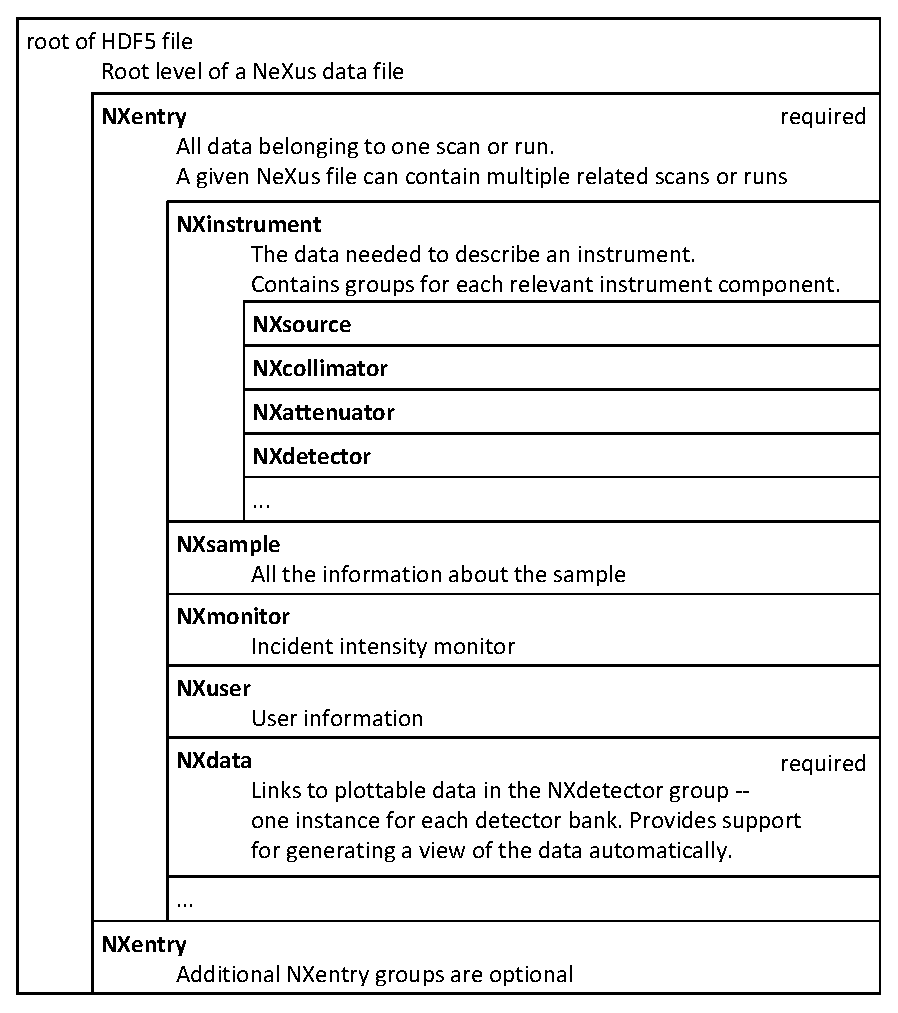
\includegraphics{figure1.eps}
\caption{\label{rawfile}Overview of the structure of a NeXus raw data file. Note that only a small part of this structure (the first \textit{NXentry} group and the first \textit{NXdata} group) is actually required.  The other content is optional.
}
\end{figure}

\begin{figure}
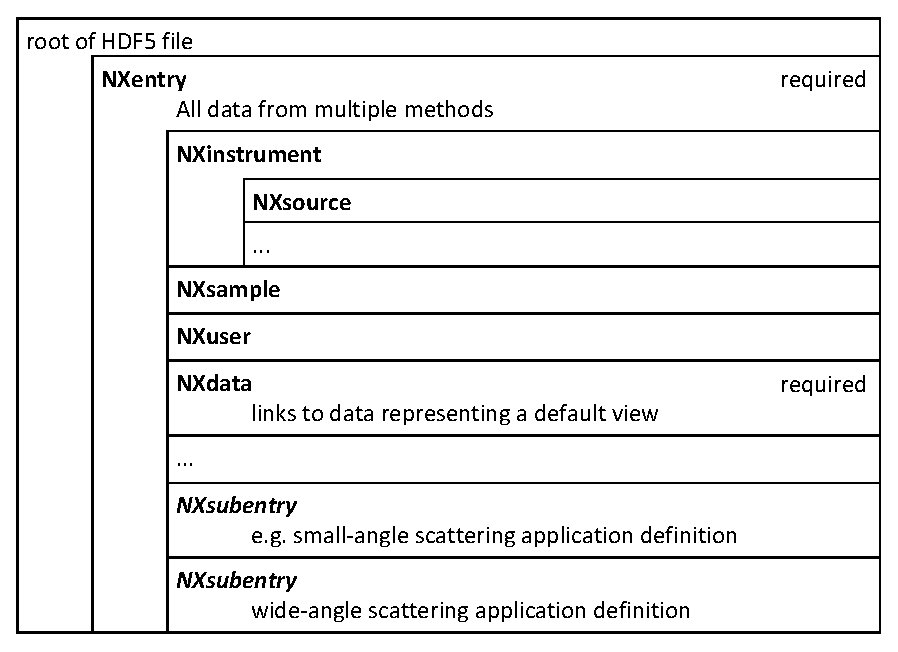
\includegraphics{figure2.eps}
\caption{\label{multimethod}Overview of the structure of a NeXus raw data file for an instrument with multiple methods.}
\end{figure}

\begin{figure}
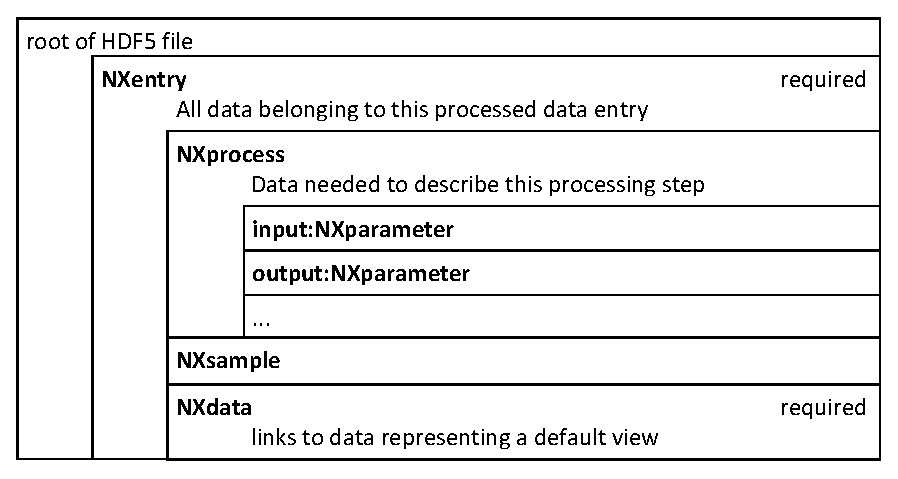
\includegraphics{figure3.eps}
\caption{\label{procfile}Overview of the structure of a NeXus processed data file.}
\end{figure}

\referencelist[nexus14aip]

\end{document}                    % DO NOT DELETE THIS LINE
%%%%%%%%%%%%%%%%%%%%%%%%%%%%%%%%%%%%%%%%%%%%%%%%%%%%%%%%%%%%%%%%%%%%%%%%%%%%%%
